\documentclass[../TDE6_rsf.tex]{subfiles}%

\begin{document}
% TODO: Reprendre correction en prenant la partie imaginaire. Cf. rM, notes
% rapides, page 8, tag "todo".
\section[s]"3"{Déphasage, pulsation et impédance}
\QR{%
	\begin{minipage}[t]{0.55\linewidth}
		On considère le circuit ci-contre en RSF. Déterminer l'expression de la
		pulsation $w$ de la tension sinusoïdale $e(t) = E\cos(\wt)$ pour que le
		courant $i(t)$ soit en phase avec $e(t)$.
		\bigbreak
		\textit{Indication}~: utiliser l'impédance équivalente constituée de $C$,
		$L$ et $R_2$.
	\end{minipage}
	\hfill
	\begin{minipage}[t]{0.40\linewidth}
		\vspace{0pt}
		\begin{center}
			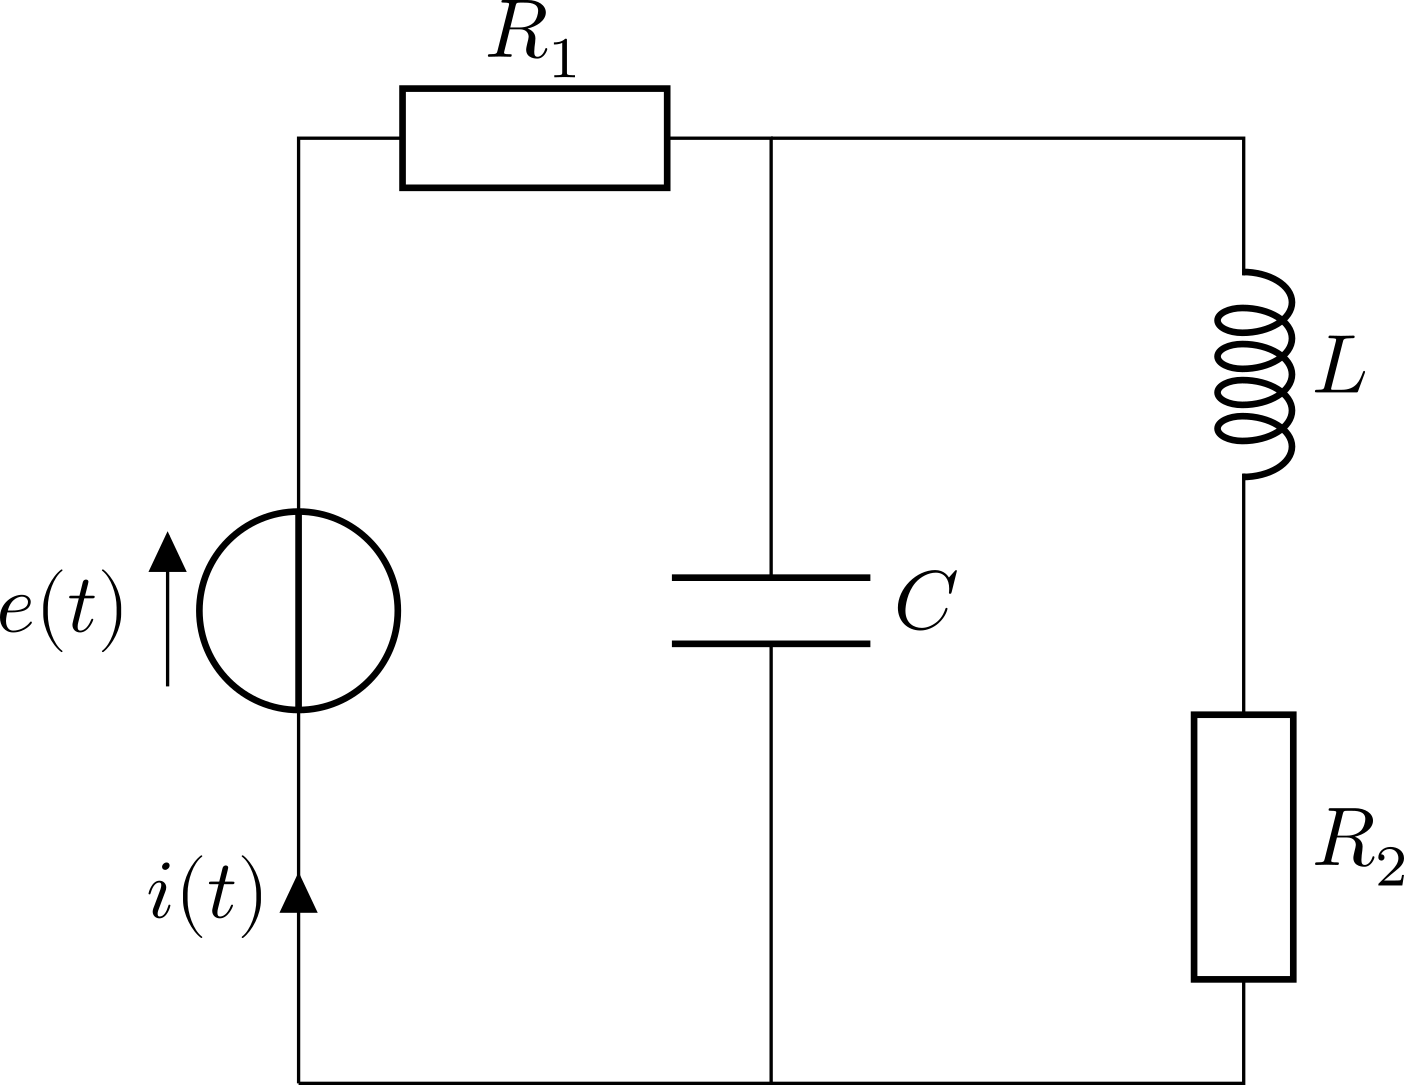
\includegraphics[width=\linewidth]{exo7_plain}
		\end{center}
	\end{minipage}
}{%
	Pour exprimer simplement $i$, il nous faut une seule maille avec une seule
	impédance équivalente $\Zu\ind{eq}$~: de cette manière, la loi des mailles nous
	donnera $\Eu = \Zu\ind{eq}\xul{I}$ et on pourra facilement déterminer le
	déphasage entre $i$ et $e$. \bigbreak
	On calcule l'impédance équivalente de l'association en série de $R_2$ et $L$~:
	\[\Zu\ind{eq,1} = R_2 + \jj L\w\]
	Cette association est en parallèle avec $C$~:
	\begin{gather*}
		\Zu\ind{eq, 2}
		= \frac{\Zu_C\times\Zu\ind{eq, 1}}{\Zu_C + \Zu\ind{eq,1}}
		= \frac{\dfrac{1}{\jj C\w}(R_2 + \jj L\w)}{\dfrac{1}{\jj C\w} + R_2 +
			\jj L\w}\\
		\Lra
		\Zu\ind{eq,2} = \frac{R_2 + \jj L\w}{1+\jj R_2C\w - LC\w^2}
	\end{gather*}
	On a donc comme prévu avec la loi des mailles~:
	\[\boxed{\xul{I} = \frac{\Eu}{R_1 + \Zu\ind{eq,2}}}\]
	L'intensité est en phase avec la tension si $\arg{R_1 + \Zu\ind{eq,2}} = 0$,
	c'est-à-dire si
	\begin{align*}
		\arg*{R_1 + \frac{R_2 + \jj L\w}{1 + \jj R_2C\w - LC\w^2}}
		 & = 0                                                   \\
		\Lra
		\arg*{\frac{R_1 + \jj R_1R_2C\w - LCR_1\w^2 + R_2 + \jj L\w}
			{1 + \jj R_2 C\w - LC\w^2}}
		 & = 0                                                   \\
		\Lra
		\arg*{(R_1 + R_2 - LCR_1\w^2) + \jj(R_1R_2C\w + L\w)}
		 & = \arg*{(1-LC\w^2) + \jj R_2C\w}                      \\
		\Lra
		\tan (\arg*{(R_1 + R_2 - LCR_1\w^2) + \jj(R_1R_2C\w + L\w)})
		 & = \tan(\arg{(1-LC\w^2) + \jj R_2C\w} )                \\
		\Lra
		\frac{R_1R_2C\w + L\w}{R_1 + R_2 - LCR_1\w^2}
		 & = \frac{R_2C\w}{1-LC\w}                               \\
		\Lra
		\frac{R_1 + \dfrac{L\cancel{\w}}{R_2C\cancel{\w}}}{R_1 + R_2 - LCR_1\w^2}
		 & = \frac{1}{1-LC\w^2}                                  \\
		\Lra
		\left( R_1 + \frac{L}{R_2C} \right) \left( 1-LC\w^2 \right)
		 & = R_1 + R_2 - LCR_1\w^2                               \\
		\Lra
		\cancel{R_1} - \bcancel{LCR_1\w^2} + \frac{L}{R_2C} - \frac{L^2\w^2}{R_2}
		 & = \cancel{R_1} + R_2 - \bcancel{LCR_1\w^2}            \\
		\Lra
		L
		 & = R_2{}^2 C + L^2C\w^2                                \\
		\Lra
		\w^2
		 & = \frac{1}{LC} - \frac{R_2{}^2}{L^2}                  \\
		\Lra
		\Aboxed{\w^2
		 & = \frac{1}{LC} \left( 1 - \frac{R_2{}^2C}{L} \right)}
	\end{align*}
}
\end{document}
